\documentclass[sigconf]{acmart}

% Metadata
\title{Time Synchronization via Remote Sensing Using Audio Events}
\author{Aidan Flood}
\affiliation{\institution{University of Massachusetts Amherst}}
\email{atflood@umass.edu}

\usepackage{graphicx}
\usepackage{amsmath}
\usepackage{listings}
\usepackage{caption}
\usepackage{subcaption}
\usepackage{float}

\lstset{basicstyle=\ttfamily\footnotesize,breaklines=true}

\begin{document}

\begin{abstract}
Precise time synchronization between distributed embedded devices is critical in applications such as event correlation, distributed sensing, and coordinated actuation. This project proposes a GPIO UART-based time synchronization system that utilizes environmental stimuli, specifically audio events, to align clocks between two ESP32 embedded devices. These devices are connected to a central Raspberry Pi 5 node which acts as the coordination and analysis hub. I introduce a passive sensing-based synchronization approach that could be transfered to a wireless protocol, such as Bluetooth Low-Energy (BLE). This design provides a low-cost, scalable alternative for temporal alignment in sensor networks.
\end{abstract}

\maketitle

\section{Introduction}
\subsection{Motivation}
Modern distributed sensing systems, particularly in IoT and embedded contexts, depend on precise time synchronization to align and fuse temporally disparate sensor data. Applications such as acoustic localization, beamforming arrays, and synchronized environmental monitoring require sub-millisecond accuracy across nodes. However, off-the-shelf embedded systems often lack access to wired synchronization infrastructure such as Precision Time Protocol (PTP) or GPS, making synchronization difficult in low-power, wireless, or use cases with poor infrastructure.

\subsection{Problem Statement}
The core problem addressed in this work is the lack of reliable, accurate, and infrastructure-independent time synchronization among multiple low-cost embedded sensor nodes. Traditional synchronization protocols either require more advanced hardware, that may be too expensive for the particular use case, or rely on wireless protocols like BLE that can suffer from unpredictable latency, connection instability, and software stack jitter. This introduces new, potentially unaccountable factores. I aim to design a synchronization system that avoids these pitfalls while still using widely available hardware like the ESP32 and Raspberry Pi.

\subsection{System Specifications}
My system includes two ESP32 microcontrollers and one Raspberry Pi 5. Each ESP32 is connected to an electret microphone and samples ambient audio using its onboard ADC. Each sample buffer is timestamped with the ESP32’s local clock and transmitted to the Raspberry Pi 5 via a UART serial connection. The Pi correlates incoming audio signals from both ESP32s to determine clock offset and synchronization drift over time. The system operates on the following specifications:
\begin{itemize}
  \item Audio sampled at 1 kHz from both ESP32 devices.
  \item Each ESP32 collects 1-second buffers (1000 samples).
  \item Data is timestamped locally and sent via UART over GPIO (115200 baud).
  \item Synchronization error is estimated using cross-correlation of audio events.
\end{itemize}

\section{Related Work}
Achieving precise time synchronization in resource-constrained embedded systems has been an active area of research, particularly for applications in sensor fusion, localization, and distributed control. 

Sandha et al. \cite{sandha2019smartphone} present an extensive study on smartphone synchronization using various peripheral interfaces such as audio, Bluetooth Low Energy (BLE), and Wi-Fi. Their work highlights the trade-offs in timestamping fidelity and peripheral stack delays, concluding that audio-based synchronization can offer sub-millisecond precision by using receiver-to-receiver (R2R) methods. My work is inspired by their finding that audio synchronization outperforms BLE and Wi-Fi in local settings due to more deterministic stack behavior and access to kernel-level timestamping in some systems.

BLE-based synchronization protocols such as CheepSync \cite{sridhar2016cheepsync} are optimized for ultra-low-power systems and advertise time information in BLE advertising packets. However, these systems suffer from unpredictable latency due to their reliance on high-level software stacks and limited control over the BLE transmission layer. In practice, my experiments with BLE revealed issues including packet loss, unstable pairing, and timing jitter, which motivated my switch to UART for more deterministic communication.

Other common approaches to synchronization in embedded networks include sender-to-receiver protocols such as NTP and IEEE 1588 PTP. However, these require either internet connectivity (NTP) or hardware timestamping capabilities (PTP), which are unavailable on the ESP32. While previous works in wireless sensor networks (WSNs) such as RBS \cite{elson2002fine} and TPSN \cite{ganeriwal2003timing} offer lightweight solutions, they still require packet exchange and propagation delay estimation, which are prone to variation.

In contrast, my method leverages ambient environmental signals, specifically audio, as naturally shared reference events. This eliminates the need for direct packet exchange between embedded nodes. Related acoustic-based time synchronization systems have also been studied for ultrasonic localization \cite{lazik2015ultrasonic}, which use precisely timed beacons. However, my system operates passively, using arbitrary ambient audio events such as music or claps, and requires no pre-scheduled transmission.

This work positions itself at the intersection of embedded sensing and infrastructure-free synchronization. By combining cross-correlation with timestamped sensor data and low-overhead UART links, I extend the ideas of audio-based synchronization into a microcontroller-driven architecture suitable for decentralized deployments.

\section{Background and Problem Context}

Precise time synchronization is foundational to many distributed sensing and control systems. In wireless sensor networks, applications such as source localization, event detection, and collaborative sampling require all nodes to maintain a shared sense of time. Traditional approaches, such as the Network Time Protocol (NTP) or Precision Time Protocol (PTP), are unsuitable for low-cost microcontrollers due to their dependence on network interfaces, hardware timestamping, or external connectivity.

Receiver-to-receiver (R2R) synchronization techniques offer an alternative. Instead of transmitting timestamped packets, nodes independently observe a shared reference event in the environment and use this event to align their local clocks. The observed event can be audio, light, or any physical stimulus that propagates across space. This method eliminates uncertainties associated with transmission and reception delays, and is particularly appealing for embedded systems where high-precision clocks or deterministic communication stacks are not available.

The ESP32 microcontroller, while versatile and widely adopted, does not support hardware timestamping or IEEE 1588. Bluetooth Low Energy (BLE), though supported, introduces substantial variability in timing due to its software stack and power-saving mechanisms. These challenges necessitate an alternative method that works within the ESP32’s constraints and still delivers practical synchronization accuracy.

\subsection{Problem Statement}
The problem addressed in this work is the design and evaluation of a time synchronization mechanism that can be deployed on low-cost microcontroller platforms without specialized hardware or dependency on unreliable wireless connections. Specifically, I aim to:
\begin{itemize}
    \item Achieve synchronization using only the onboard clocks and sensors of ESP32 devices.
    \item Leverage ambient signals such as audio as a naturally shared time reference.
    \item Enable clock offset estimation using minimal hardware and robust computation.
\end{itemize}

\noindent In the following section, I describe the architecture and mechanisms of my proposed solution.

\section{System Design}
Figure~\ref{fig:system-diagram} illustrates my high-level system architecture for audio-based time synchronization between embedded devices.

\begin{figure}[H]
    \centering
    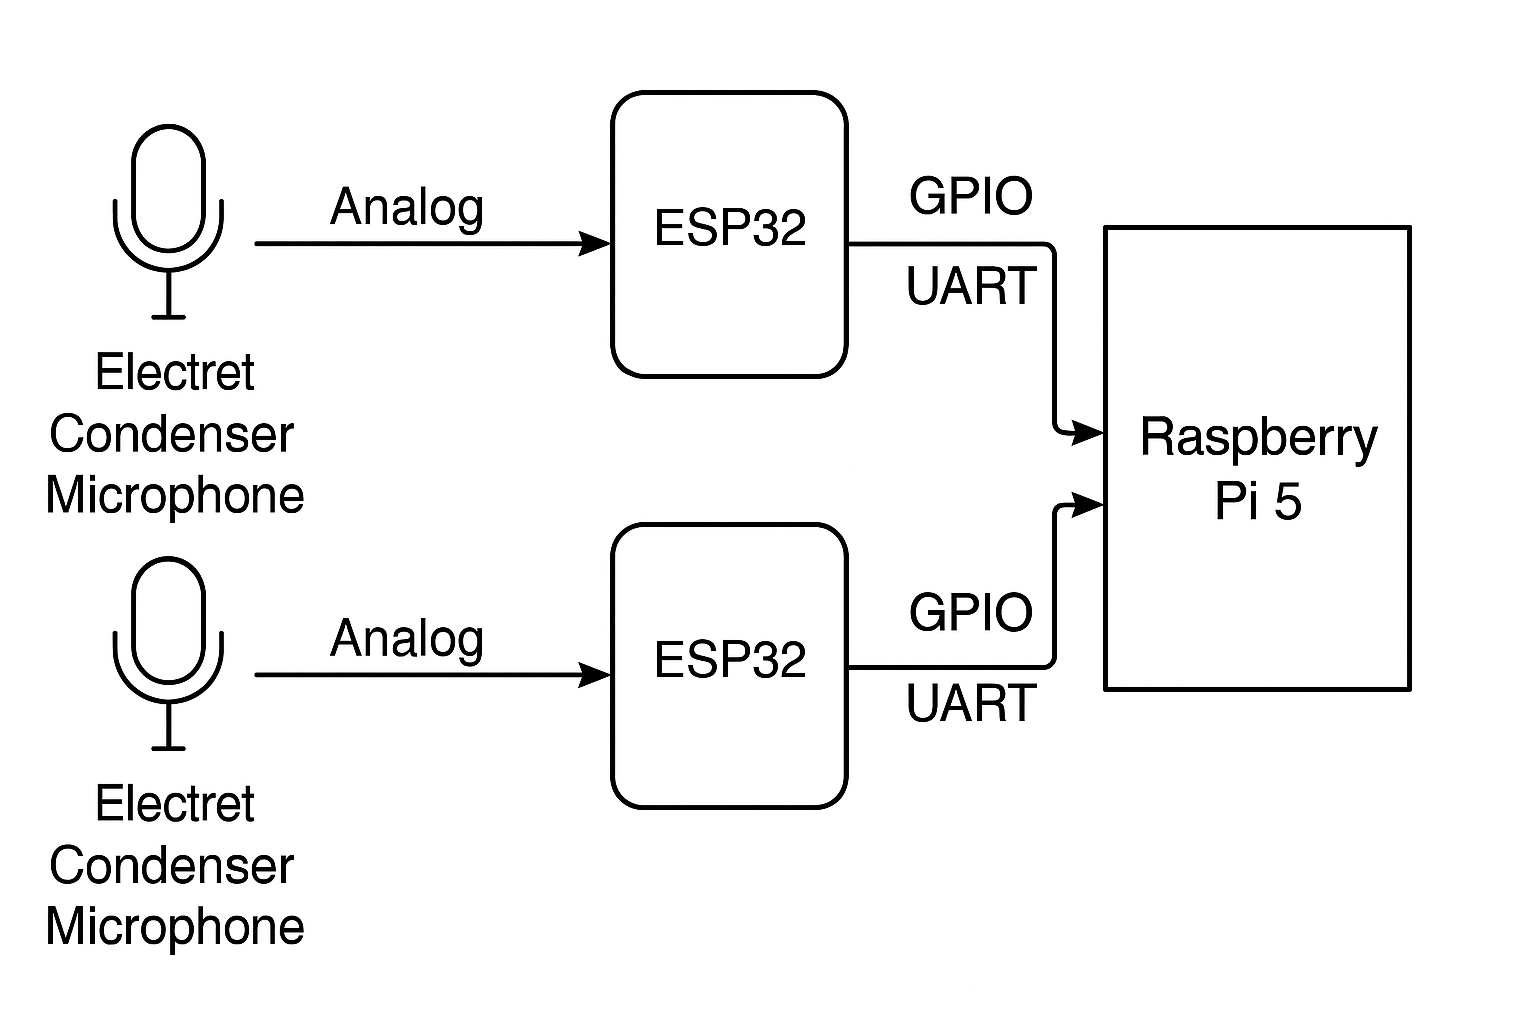
\includegraphics[width=\linewidth]{system_diagram.png}
    \caption{System architecture: ambient audio is sensed by microphones connected to ESP32s, which forward timestamped samples to the Raspberry Pi 5 via UART for correlation and time offset estimation.}
    \label{fig:system-diagram}
\end{figure}

The system follows a \textbf{receiver-to-receiver} (R2R) synchronization model. A shared environmental signal—ambient audio—is sensed independently by two ESP32 nodes using electret microphones. These analog signals are sampled by each ESP32’s ADC at a fixed sampling rate (e.g., 1 kHz). Each ESP32 timestamps its own samples using its internal clock, creating a local view of the audio waveform.

The Raspberry Pi 5 functions as the central coordinator. At regular intervals, it sends a UART request to each ESP32. In response, each ESP32 transmits a buffer of recent samples alongside the associated timestamp. The Pi then computes the cross-correlation between the two buffers to find the sample-wise offset at which the waveforms best align. This offset directly reflects the difference in local time between the two ESP32s, enabling synchronization.

\subsection{Architectural Contributions}
Unlike many systems that rely on packet-based sender-to-receiver synchronization over high-latency wireless links (BLE or Wi-Fi), my approach uses \textbf{passive sensing of shared environmental events}, which are naturally present in many real-world environments. The technical novelty lies in the application of this R2R strategy to low-cost embedded systems without reliance on specialized hardware like PTP-capable NICs.

Additionally, the use of cross-correlation for clock offset estimation in a UART-connected system avoids packet timestamping entirely. It leverages analog sensor data—audio waveforms—rather than digital handshakes, simplifying the protocol and reducing susceptibility to jitter or software stack delays.

\subsection{Design Tradeoffs}
\begin{itemize}
    \item \textbf{UART vs BLE:} BLE was originally considered due to its wireless nature but exhibited instability in maintaining long-term connections, unpredictable latency, and complexity in reconnection logic. UART, while wired, provided consistent and low-latency data transfer, making it more suitable for a robust prototype.
    \item \textbf{Audio vs Other Modalities:} Audio events (e.g., music, claps) are relatively easy to generate and detect. Other sensors like light or IMUs were tested but produced noisier or less reliably synchronous signals. However, they could be combined with audio to increase confidence in synchronization using sensor fusion.
    \item \textbf{No Global Clock:} The system deliberately avoids attempting to compute absolute time. Instead, it maintains \textit{relative synchronization}, which is sufficient for many applications like spatially-aware sensing and coordinated sampling.
\end{itemize}

This architecture emphasizes reliability and clarity over complexity, and demonstrates that even basic microcontrollers can achieve millisecond-scale synchronization through shared physical stimuli.


\section{Implementation}

This section describes the hardware and software components used to implement my synchronization system, along with the rationale behind the choice of platform and configuration for testing.

\noindent\textbf{GitHub Repository:} Source code, configuration files, and figures for this project can be accessed at: \\ \url{https://github.com/aflood37/ECE635_TimeSynchronization}


\subsection{Hardware}
\begin{itemize}
    \item \textbf{ESP32 WROOM Modules:} These microcontrollers serve as the sensor nodes. Each unit samples analog audio through an electret microphone circuit that includes an op-amp to amplify the signal to a suitable ADC range. The ESP32 was chosen for its low power usage, built-in ADC, and flexible UART communication.
    \item \textbf{Electret Microphones:} These serve as the primary sensors. Positioned near a common audio source (e.g., a speaker), the microphones detect ambient events that propagate to both ESP32s.
    \item \textbf{Raspberry Pi 5:} Functions as the synchronization server. It connects to both ESP32s via two independent GPIO UART channels. The Pi 5 was selected due to its multi-UART capability, compute power for signal processing (e.g., numpy-based correlation), and compatibility with Linux-based development.
\end{itemize}

\subsection{Testbed Setup}
The testbed consists of a fixed audio source such as a desktop speaker playing repeatable acoustic signals (e.g., clicks, tones, or music). Each ESP32 is placed at approximately equal distances from the source to ensure similar signal propagation delays. The microphones are positioned to maximize clarity and reduce noise artifacts.

The Pi and ESP32s are powered independently to eliminate shared ground effects and emulate a more realistic deployment scenario. The entire setup operates on a benchtop, with audio stimuli triggered manually or through a script, and the resulting logs and plots are saved on the Pi for offline analysis.

This testbed is ideal for prototyping as it:
\begin{itemize}
    \item Allows rapid iteration on firmware and daemon updates.
    \item Supports controlled audio inputs for repeatable testing.
    \item Provides easy access to real-time logs and live plotting tools.
    \item Mirrors a scalable topology for future extensions (e.g., adding more ESP32s or multiple modalities).
\end{itemize}

\subsection{Software}

The implementation includes tightly integrated firmware for the ESP32 nodes and a Python-based daemon that runs on the Raspberry Pi 5.

\textbf{ESP32 Firmware (main.ino)}
\begin{lstlisting}[language=C++,caption=ESP32 sampling loop]
void loop() {
  if (Serial.available()) {
    String cmd = Serial.readStringUntil('\n');
    if (cmd.startsWith("SYNC")) {
      uint32_t ts = millis();
      Serial.write((uint8_t*)&ts, sizeof(ts));
      for (int i = 0; i < N; i++) {
        uint16_t sample = analogRead(MIC_PIN);
        Serial.write((uint8_t*)&sample, sizeof(sample));
        delayMicroseconds(SAMPLING_INTERVAL);
      }
    }
  }
}
\end{lstlisting}

The ESP32 firmware waits for a SYNC command from the Pi over UART. Upon receiving the command, it timestamps the current moment and captures a fixed-length buffer of ADC samples at a set interval (typically 1 kHz). These samples are streamed back in binary format to reduce latency and overhead.

\textbf{Raspberry Pi Daemon (Python)}
The daemon is implemented in Python using multiple threads to manage data acquisition concurrently from the two UART-connected ESP32s. It relies on two main modules:
\begin{itemize}
    \item \texttt{esp\_device.py}: A class that abstracts serial communication, handles retries, validates buffer completeness, and reads binary-encoded timestamped sample data.
    \item \texttt{time\_sync\_daemon.py}: Initializes serial connections, launches concurrent readers, performs signal alignment via cross-correlation, and visualizes/logs clock offset history.
\end{itemize}

\begin{lstlisting}[language=Python,caption=Serial reader snippet]
def read_samples(self):
    base_ts_bytes = self.ser.read(4)
    base_ts = int.from_bytes(base_ts_bytes, 'little')
    data = self.ser.read(2 * N)
    samples = np.frombuffer(data, dtype=np.uint16)
    return base_ts, samples
\end{lstlisting}

\begin{lstlisting}[language=Python,caption=Cross-correlation for offset estimation]
def estimate_offset(samples1, samples2):
    corr = np.correlate(samples1 - np.mean(samples1),
                        samples2 - np.mean(samples2), mode='full')
    lag = np.argmax(corr) - (len(samples1) - 1)
    offset_ms = lag * SAMPLING_INTERVAL_MS
    return offset_ms, corr
\end{lstlisting}

The daemon also includes real-time plotting using Matplotlib, which enables live monitoring of offset drift and correlation strength. Logging is performed to both a human-readable `.log` file and structured CSV for analysis.

The software is modular and extensible, designed to be refactored into a system service for continuous operation. The use of threading, buffered I/O, and lightweight numeric computation makes it suitable for real-time embedded deployment.

Together, this hardware-software ecosystem forms a robust and repeatable prototype environment for testing low-cost time synchronization techniques using ambient sensing.

\section{Evaluation}

To evaluate the performance of my synchronization system, I used several metrics including estimated clock offset stability, correlation strength, and signal alignment before and after applying offset corrections.

My system uses a sampling rate of 1 kHz, which theoretically limits temporal resolution to 1 millisecond. Under ideal conditions, this sets a hard lower bound on the achievable synchronization error. In practice, I achieve alignment accuracy close to this bound, with estimated offsets varying within a narrow band once initial convergence is reached.

\subsection{Results}
\subsubsection{Clock Offset History}
Figure~\ref{fig:offset-history} shows the estimated clock offset between the two ESP32 devices over time. Despite initial fluctuations during startup, the offset stabilizes near 5.368 ms, indicating that the system successfully maintains consistent synchronization across successive sample windows.

\begin{figure}[H]
    \centering
    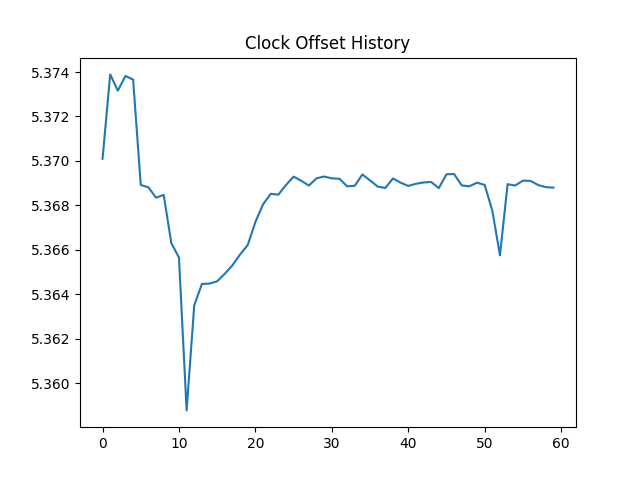
\includegraphics[width=0.8\linewidth]{offset_history.png}
    \caption{Clock Offset History: Offset convergence and stability over time between ESP32 devices.}
    \label{fig:offset-history}
\end{figure}

\subsubsection{Correlation Strength}
Figure~\ref{fig:correlation-history} plots the correlation magnitude (on a logarithmic scale) for each measurement interval. High values signify strong alignment of observed events. Outliers with low correlation are easily identifiable and may be filtered to improve offset stability.

\begin{figure}[H]
    \centering
    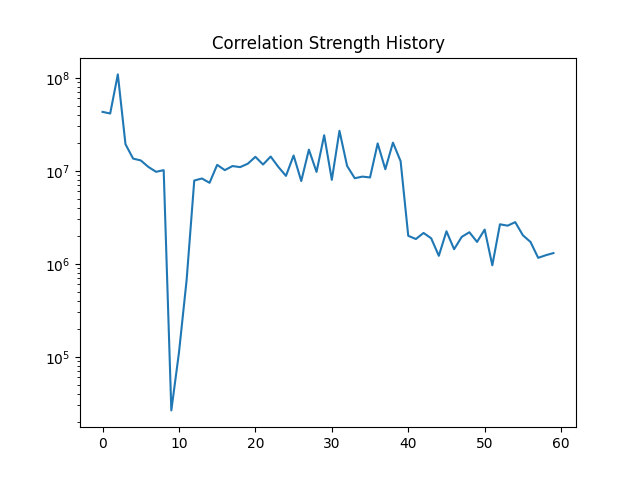
\includegraphics[width=0.8\linewidth]{correlation_history.png}
    \caption{Correlation Strength History: Peaks indicate confident synchronization events.}
    \label{fig:correlation-history}
\end{figure}

\subsubsection{Signal Alignment}
To visually validate alignment, I plotted overlapping raw ADC samples from both ESP32s before and after applying the offset correction. Figure~\ref{fig:signal-alignment} shows that once corrected, the audio waveforms match closely.

\begin{figure}[H]
    \centering
    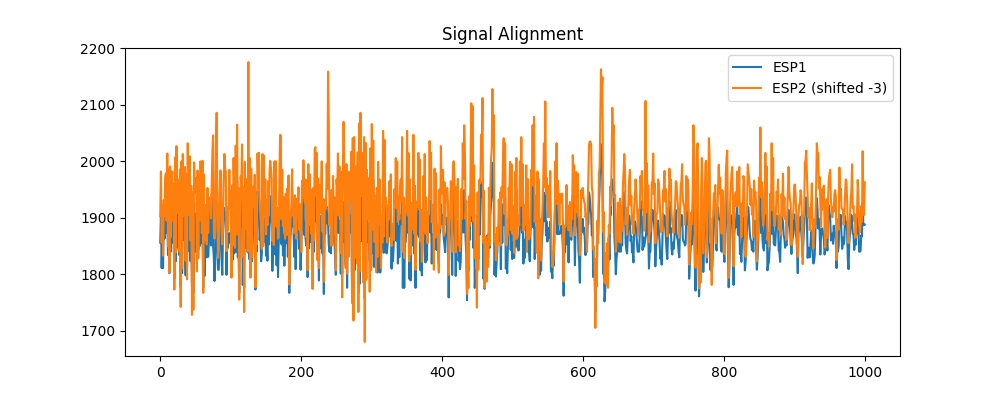
\includegraphics[width=\linewidth]{signal_alignment.png}
    \caption{Signal Alignment: ESP2 samples are shifted by -3 ms to match ESP1's waveform.}
    \label{fig:signal-alignment}
\end{figure}

\subsection{Discussion}
I observed that the system could consistently resolve offsets down to approximately 1 ms, which matches the theoretical limit imposed by the sampling rate. If a more advanced filtering or smoothing protocol were used—such as exponential averaging or Kalman filtering—offset estimation could become more robust to transient outliers and jitter.

The correlation-based approach proved sensitive and efficient for alignment, especially when sharp acoustic events were present. Weak or noisy events occasionally resulted in low-confidence measurements, highlighting the need for multi-modal validation in future iterations.

\textbf{Limitations and Lessons Learned:}
\begin{itemize}
    \item \textbf{Noisy Sensor Data:} The system’s reliance on raw microphone input made it susceptible to environmental noise, particularly in uncontrolled settings. This occasionally caused misleading correlation peaks and offset estimates.
    \item \textbf{Static Offset Application:} The current implementation applies the most recent correlation-based offset directly to align signals. This made the system responsive to outliers and introduced jitter. A stateful offset estimator would be more stable.
    \item \textbf{BLE Instability:} BLE was originally used for data transmission, but persistent issues with packet fragmentation and connection drops made it impractical. This highlighted the benefit of simpler, lower-layer protocols like UART.
    \item \textbf{Limited Sampling Resolution:} A 1 kHz sampling rate limits temporal precision to 1 ms. While sufficient for this proof of concept, finer resolution would require either higher sampling rates or interpolation techniques.
    \item \textbf{Manual Triggering:} Audio events were triggered manually (e.g., music or claps), which limited testing repeatability. Automating the stimulus source would support more systematic validation.
    \item \textbf{Debugging UART and Timing Drift:} UART-based communication was ultimately reliable, but edge cases like incomplete buffers or misaligned timestamps required careful handling and retries in the daemon.
\end{itemize}

Overall, this implementation demonstrated that low-cost, off-the-shelf components can support millisecond-scale synchronization using shared environmental signals. It also underscored the importance of robust communication, signal quality, and statistical filtering in building dependable distributed systems.


\section{Conclusion}

This project presents a practical, low-cost approach to time synchronization between embedded devices using ambient audio and a receiver-to-receiver model. By leveraging shared acoustic events and correlating timestamped audio samples from distributed ESP32 nodes, I demonstrate that synchronization accuracy on the order of 1 millisecond is achievable using standard hardware components and UART communication.

The system achieves its goal of demonstrating reliable relative synchronization in a decentralized sensing environment. The Raspberry Pi 5 effectively coordinates data collection and performs offset estimation through efficient correlation processing. Despite limited sampling resolution and occasional correlation outliers, the system consistently converged to a stable offset profile under controlled audio stimuli.

Beyond validating this design, the project uncovered important tradeoffs and lessons in communication reliability, signal integrity, and protocol design. The final solution favored simplicity and determinism over wireless flexibility, choosing UART over BLE after encountering instability in BLE stack behavior.

\subsection{Future Directions}
Building on this foundation, several enhancements and extensions are possible:
\begin{itemize}
    \item \textbf{Sensor Fusion:} Integrating multiple sensing modalities (e.g., light, IMU) could enhance robustness, particularly in noisy or unpredictable environments.
    \item \textbf{Dynamic Offset Filtering:} Implementing filters such as exponential moving averages or Kalman filters can smooth offset estimates and reduce jitter from spurious correlations.
    \item \textbf{Automated Event Generation:} Deploying controlled stimulus generators (e.g., tone beacons) would improve test repeatability and allow stress testing under known signal conditions.
    \item \textbf{Higher Sample Rates:} Increasing the ADC sampling rate could push the synchronization resolution beyond 1 ms and support more precise applications such as audio beamforming.
    \item \textbf{Scalability:} Expanding the architecture to handle three or more ESP32 devices would test its scalability and identify bottlenecks in multi-device coordination.
    \item \textbf{Deployment as a Service:} Packaging the time synchronization daemon as a system service would support long-running deployment on embedded Linux systems.
\end{itemize}

This project demonstrates that accurate time alignment is possible without external time references or advanced hardware. Through lightweight signal processing and environmental sensing, embedded systems can synchronize reliably in real-world settings—a promising step toward autonomous, decentralized sensor networks.

\noindent\textbf{GitHub Repository:} Source code, configuration files, and figures for this project can be accessed at: \\ \url{https://github.com/aflood37/ECE635_TimeSynchronization}


\bibliographystyle{ACM-Reference-Format}
\bibliography{references}

\end{document}
